\documentclass[a4paper,12pt]{article}
\usepackage[slovene]{babel}
\usepackage[utf8]{inputenc}
\usepackage[T1]{fontenc}
\usepackage{lmodern}
\usepackage{amsmath,amsfonts}
\usepackage{enumitem}
\usepackage{graphicx}
\usepackage{subfigure}
\usepackage{mathtools}
\pagenumbering{roman}

\begin{document}

\newcommand{\N}{\mathbb{N}}
\newcommand{\R}{\mathbb{R}}
\newcommand\sbullet[1][.5]{\mathbin{\vcenter{\hbox{\scalebox{#1}{$\bullet$}}}}}
%\theoremstyle{definition} % tekst napisan pokoncno
\newtheorem{definicija}{Definicija}[section]
\newtheorem{primer}[definicija]{Primer}
\newtheorem{opomba}[definicija]{Opomba}

\title{Diskretne Coonsove ploskve}
\author{Matej Rojec, Vito Rozman}
\date{\today}

\maketitle


\newpage

\tableofcontents
\listoffigures

\newpage

\section{Uvod}

V seminarski nalogi bomo obravnavali ploskve, ki interpolirajo štiri mejne krivulje,
ki so definirane vsaka na svoji stranici pravokotnika $[0,1]^2$. 
Te ploskve bomo imenovali diskretne Coonsove ploskve, 
ki jih bomo dobili z reševanjem linearnega sistema enačb.
Pogledali si bomo tudi problem, ko imamo namesto pravokotnika podan 
trikotnik, ki ga interpolirajo tri merjne krivulje.


Eden od najstarejših problemov v Računalniško podprtem geometrijskem oblikovanju je problem, 
kjer imamo podane štiri robne krivulje, radi pa bi poiskali ploskev z danimi robnimi krivuljami. 
Torej podane imamo robne krivulje $$x(u,0), x(u,1), x(0,v),  x(1,u),$$ kjer lahko brez škode za 
splošnost predpostavimo da je domena ploskve $x(u,v)$ enotni kvadrat, torej $(u,v) \in [0,1]^2$. 
Znana rešitev tega problema je bilinearna mešana Coonsova ploskev, ki je interpolirana z robnimi 
krivuljami, kot: 
\begin{align*}
   \label{continiusCons}
   \mathbf{x}(u,v) =& (1-u)x(0,v) +ux(1,v)\\
    & + (1-v)x(u,0) +vx(u,v) \\
   & - 
   \begin{bmatrix} 
      1-u & u 
   \end{bmatrix}
   \begin{bmatrix} 
      x(0,0)& x(0,1)\\
      x(1,0)& x(1,1) 
   \end{bmatrix}
   \begin{bmatrix}
      1-v\\
      v
   \end{bmatrix}
\end{align*}


\section{Diskretne Coonsove ploskve}
V bolj modernih uporabah RPGO, so mejne krivulje Bézierjeve polinomske krivulje, 
ki jih napenjajo kontrolne točke. 
\begin{definicija}
    Naj bodo dane kontrolne točke $\mathbf{b}_0, \mathbf{b}_1, \dots, \mathbf{b}_n \in \R^d$. 
    Potem je Bézierjeva krivulja stopnje $n$ podana s polinomsko paramerizacijo $\mathbf{p}: [0,1] \rightarrow \R^d$ s predpisom 
    $$\mathbf{p}(t) = \sum_{i=0}^n \mathbf{b}_{i} B_i^n(t),$$
    kjer je $B_i^n(t) = \binom{n}{i} t^i (1-t)^{n-i}$, za $i = 0, 1,\dots,n$. 
   % Točkam $\mathbf{b}_i$ pravimo kontolne točke.
\end{definicija}

% kle manjka nek vezni tekst med definicijama
Podobno lahko definiramo Bézierjeve ploskve na sledeč način.

\begin{definicija}
    Bézierjevo ploskev $\mathbf{p} : [0,1]^2 \rightarrow \R^3$ iz tenzorskega produkta stopnje 
    $(m, n) \in \N \times \N$ definiramo s parametrizacijo:
    $$\mathbf{p}(u,v) := \sum_{i=0}^m \sum_{j=0}^n \mathbf{b}_{i,j} B_i^m(u)B_j^n(v),$$
    kjer sta $(u,v) \in [0,1]^2$ ter $(\frac{i}{m}, \frac{j}{n})$
    domenske točke, ki ustrezajo kontrolni točki $\mathbf{b}_{i,j}$.
\end{definicija}


Predpostavimo, da imamo podane robne kontrolne točke $\mathbf{b}_{i,j}$ 
izračunane pri prametru $(u,v)$, ki predstavljajo sledečo shemo: 
$$
\begin{matrix}
   \mathbf{b}_{0,0}  &\mathbf{b}_{1,0} & \ldots &\mathbf{b}_{m-1,0} &\mathbf{b}_{m,0} \\
   \mathbf{b}_{0,1}  &                 &        &                   &\mathbf{b}_{m,1} \\
   \vdots            &                 &        &                   &  \vdots\\
   \mathbf{b}_{0,n-1} &                &        &                    &\mathbf{b}_{m,n-1} \\ 
   \mathbf{b}_{0,n}  &\mathbf{b}_{1,n} & \ldots &\mathbf{b}_{m-1,n} &\mathbf{b}_{m,n} 
\end{matrix}
$$

   

Sedaj lahko primer diskritiziramo in robne krivulje zapišemo s štirimi 
Bezierjevimi krivuljami:
\begin{align*}
    &\mathbf{p}(u,0) =\sum_{i=0}^m \mathbf{b}_{i,0} B_i^n(u), \qquad
    \mathbf{p}(u,1) =\sum_{i=0}^m \mathbf{b}_{i,n} B_i^n(u),  \\
    &\mathbf{p}(0,v) =\sum_{j=0}^n \mathbf{b}_{0,j} B_j^n(v), \qquad
    \mathbf{p}(1,v) =\sum_{j=0}^n \mathbf{b}_{m,j} B_j^n(v),  \\
 \end{align*}
Notranje točke kontrolnega polinoma, lahko izračunamo na podoben način kot zgoraj: 
\begin{align*}
   \mathbf{b}_{i,j} &= \left(1 - \frac{i}{m}\right)\mathbf{b}_{0,j} +\frac{i}{m}\mathbf{b}_{m,j}\\
    &+ \left(1 - \frac{j}{n}\right)\mathbf{b}_{i,0} +\frac{j}{n}\mathbf{b}_{i,n}\ \\
   &- 
   \begin{bmatrix} 
      1 - \frac{i}{m} & \frac{i}{m}
   \end{bmatrix}
   \begin{bmatrix} 
      \mathbf{b}_{0,0} & \mathbf{b}_{0,1}\\
      \mathbf{b}_{1,0} & \mathbf{b}_{1,1}
   \end{bmatrix}
   \begin{bmatrix}
      1 - \frac{j}{n}\\
      \frac{j}{n}
   \end{bmatrix}
\end{align*}
za $i = 1,2,\dots,m-1$ in $j = 1,2,\dots,n-1$. Izkaže se, da je kontrolni poligon ploskev, 
ki jo omejujejo robne krivulje, enak kontrolnemu poligonu, ki ga dobimo z opisano metodo. 
»Morda zanimivo: za določene oblike rabimo definirati samo robne krivulje«.

Ploskev, ki jo dobimo s tako dobljenimi kontrolnimi točkami $\mathbf{b}_{i,j}$
imenujemo Coonsova ploskev.

Primer take ploskve je slika \ref{fig:whatever}, kjer je prikazan 
rob kontrolnega poligona, notranje točke kontrolnega poligona in 
Bézierjeva ploskev definirana nad kontrolnim poligonom

\begin{figure}[ht!]
   \centering
   \subfigure[Primer robnih točk]{
   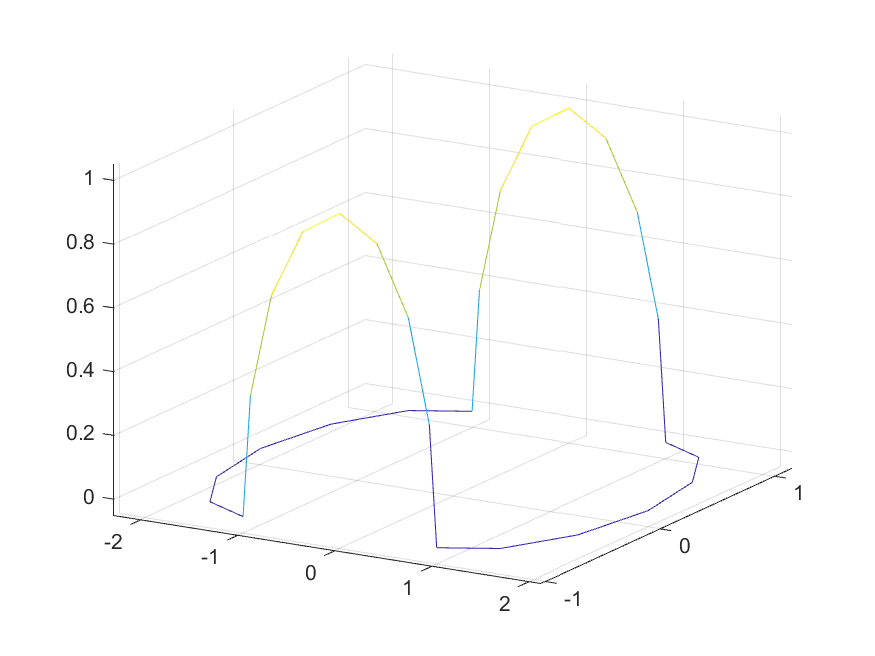
\includegraphics[width=0.45\textwidth]{ogrodje.png}
   }
   \subfigure[Primer ogrodja]{
   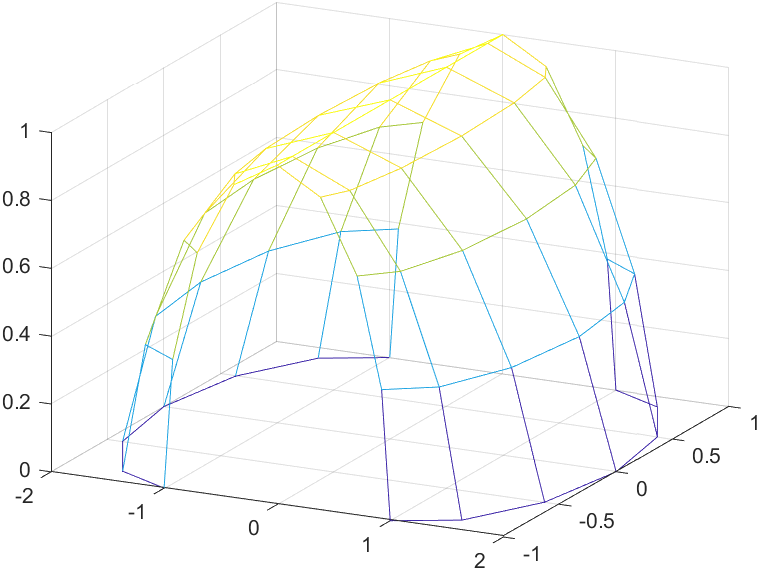
\includegraphics[width=0.45\textwidth]{dodatne_kont_t.png}
   }
   
   \subfigure[Coonsova ploskv na ogrodju]{
   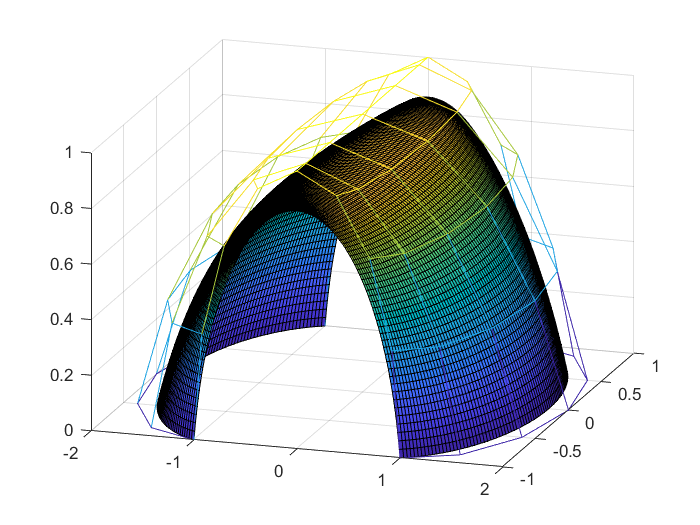
\includegraphics[width=0.5\textwidth]{primer_krivulje.png}
   }   
   \caption{Primer konstrukcije Coonsove ploskve}
\label{fig:whatever}
\end{figure}


\newpage




\section{Stalnost Coonsove ploskve}
\label{ch:3}

%\subsection{Minimziraje zasuka}
%Coonsova ploskve minimzirajo zasuk, definiran kot:
%\begin{equation}
%   \label{eq:min}
%   \int_{[0,1]^2} \left( \frac{\partial^2}{\partial u \partial v}\mathbf{p}(u,v) \right)^2 dS.
%\end{equation}
%Torej coonsova ploskev doseže minimum izraza.
%Posledica tega je, da so Coonsova ploskve lahko v primerih preveč ravne in ne interpolirajo dobro kontrolnih točk.
%Taka ploskev prav tako zadošča Euler-Lagrangovi parcialni diferencialni enačbi, torej velja:
%\begin{equation}
%   \label{eq:pde}
%    \frac{\partial^4}{\partial u^2 \partial v^2}\mathbf{p}(u,v) = 0.
%\end{equation}

Denimo, da imamo podano Cooncova ploskev definirana nad domeno $D = [0,1]^2$. 
Izberemo dve točki $(u_0,v_0)$ in $(u_1,v_1)$ ki razpenjata pravokotnik $R$ v domeni $D$. 
Štiri mejne krivulje pod-Coonsove ploskve definirae na $R$ se preslikajo 
v štiri krivulje na prvotno Coonsovo ploskev. Izkaže se da pod-Coonsova ploskev 
definirana na $R$ je prvotna Coonsova ploskev zožana na območje $R$. To načelo 
lahko uporabimo na diskretni $3 \times 3$ Coonsovi ploskivi
$$
\begin{matrix} 
   \mathbf{b}_{i-1,j-1} & \mathbf{b}_{i-1,j} & \mathbf{b}_{i-1,j+1}\\
   \mathbf{b}_{i,j-1} & \mathbf{b}_{i,j} & \mathbf{b}_{i,j+1}\\
   \mathbf{b}_{i+1,j-1} & \mathbf{b}_{i+1,j} & \mathbf{b}_{i+1,j+1}
\end{matrix}
$$ 
Če poznamo robne točke lahko notranjo točko $\mathbf{b}_{i,j}$ določimo na sledeč način: 
\begin{align*}
   \mathbf{b}_{i,j} =& -\frac{1}{4}(\mathbf{b}_{i-1,j-1} + \mathbf{b}_{i+1,j-1} +
      \mathbf{b}_{i-1,j+1} + \mathbf{b}_{i+1,j+1}) \\
      &+\frac{1}{2}(\mathbf{b}_{i-1,j} + \mathbf{b}_{i,j-1}+
      \mathbf{b}_{i,j+1} + \mathbf{b}_{i+1,j}).\\
\end{align*}
kar lahko krajše zapišemo z masko: 
$$
\mathbf{b}_{i,j} = -\frac{1}{4} \times 
\begin{matrix*}[r]
-1 && 2 && -1 \\
2 && \sbullet && 2\\
-1 && 2 && -1
\end{matrix*}
$$
Ker je mreža sestavljena iz $(m+1)\times(n+1)$ kontrolnih točk, dane pa imamo samo robne
točke lahko ostalih $(m-1)\times(n-1)$ enlično določimo z zgornjo masko. Določitev točk se prvede
na reševanje sistema $(m+1)\times(n+1)$ linearnih enačb.

Oglejmo si $3 \times 3$ masko s splošnimi parametri, kjer se element izraža na sledeč način:
$$
\mathbf{b}_{i,j} =  \quad 
\begin{matrix*}[r]
\alpha && \beta && \alpha \\
\beta && \sbullet && \beta. \\
\alpha && \beta && \alpha
\end{matrix*}
$$
V primeru da sta $(\alpha, \beta) = (-0.25, 0.5)$ dobimo Coonsovo
ploskvo. Privzeli bomo, da velja $4\alpha + 4\beta = 1$, saj 
tako ohranjamo afinost maske. S perturbiranjem parametrov 
$\alpha$ in $\beta$ dobimo torej nov razred kontrolnih shem, imenujemo jih stalne 
krivulje (angl. \textit{permanence patches}). V članku \cite{DCP}  so raziskovali
vpliv $\alpha$ na optimalno oblike ploskve. Ugotovili so, da za izbrana $m$ in $n$
ni vedno ene optimalne vrednosti za $\alpha$, ki bo dala dobro obliko ploskve.

\section{Stalne Coonsove ploskve}
\label{ch:4}

Ena kontrolna točka navadne Coonsove ploskve je odvisna od osem obrobnih točk, 
torej gre za lokalno odvisnost. V primeru ko govorimo o stalnih ploskvah 
($\alpha \neq  -0.25$), je točka odvisna od vseh mejnih točk, zato govorimo 
o globalni odvisnosti. Ta odvisnost nam potencialno lahko pripomore pri ustvarjanju 
``boljše'' krivulje.
% @Vito narekovaje se vidno v LaTeX-u piše kot sem zgoraj nakazal

Oglejmo si še nekaj primerov ploskev pri različnih parametrih $\alpha$ in $\beta$.
V primeru, da v sliki \ref{fig:whatever} pustimo ogrodje kontrolnih točk enako,
namesto parametra $\alpha =- 0.25$ pa uporabimo 
parametra $\alpha = -0.26$ ter $\alpha = -0.23$ in rešimo sistem
linearnih enačb dobimo krivulje prikazane na sliki \ref{fig:coons_pospl}.

\begin{figure}[ht!]
   \centering
   \subfigure[Stalna krivulja pridobljena s parametrom $\alpha = -0.26$]{
   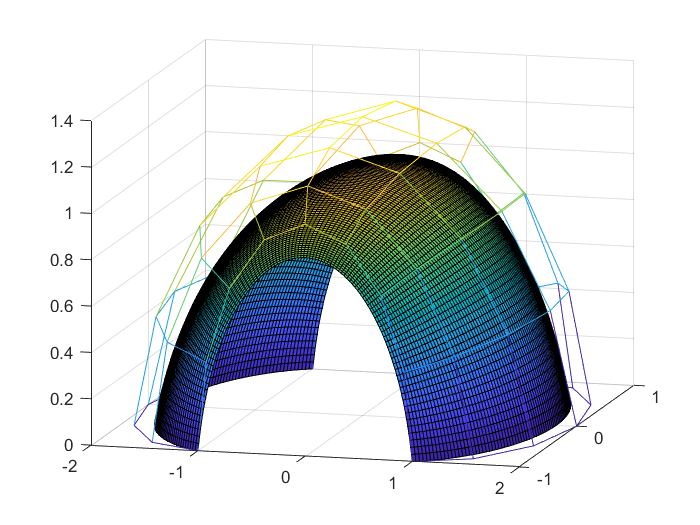
\includegraphics[width=0.45\textwidth]{square_26.png}
   }
   \subfigure[Stalna krivulja pridobljena s parametrom $\alpha = -0.26$]{
   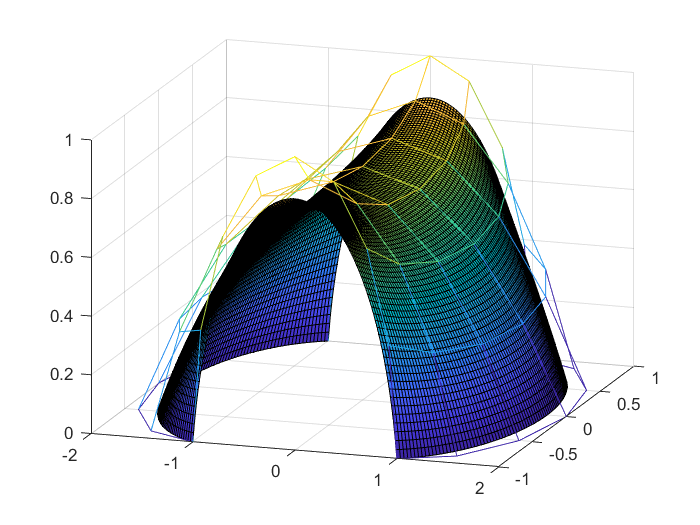
\includegraphics[width=0.45\textwidth]{square_23.png}
   }
   \caption{Stalni krivulji pridobljeni z reševanjem sistemov linearnih enačb}
\label{fig:coons_pospl}
\end{figure}






Dani poligoni izhajajo iz torusnih oblik in z modifikacijo $\alpha$ lahko pridemo do željene oblike.
Kot zanimivost se izkaže da pri izbiri paramatra $\alpha = 0$ in seveda ob upoštevanju afinosti,
dobimo ploskev, katere površina je minimizeranan za dano ogrodje krivulj. To se vidi iz Laplasove parcialne 
diferencialne enačbe
% @Vito polinomske ploskve se piše s p
$$\mathbf{p}_{uu} + \mathbf{p}_{vv} = 0.$$


\section{Trikotne stalne Coonsove ploskve}

%@Vito piecewise = odsekoma 
Oglejmo si primer, ko imamo krivulje definirane nad trikotnikom 
namesto nad pravokotnikom kot v razdelkih \ref{ch:3} in \ref{ch:4}.
Pojavi se naslednje vprašanje, če imamo podane tri robne kontrolne poligone 
ki razpenjajo zunanjost trikotnika, ali obstaja  ``dobra''
kontolna mreža, ki zapolni omejeno območje. 
Podobno kot v razdelkih \ref{ch:3} in \ref{ch:4} lahko uporabimo načelo 
stalnosti za masko:

$$
\mathbf{x} =  \quad 
\begin{matrix*}[r]
          &       &       & \alpha   &       &       & \\
          &       & \beta &          & \beta &       & \\
          & \beta &       & \sbullet &       & \beta & \\
   \alpha &       & \beta &          & \beta &       & \alpha
\end{matrix*}
$$
kjer je zaradi pogoja afinoste ponovno zahtevamo,da je $3\alpha + 6\beta = 1$.
% @Vito a je kle n nad 2 ? 
Podbono kot prej rešimo $\binom{n+1}{2}$, kjer je $n$ število kontrolnih točk 
na eni stranici trikotnika.

Na sliki \ref{fig:trikotne} vidimo tri možne oblike stalne trikotne
krpe s parametri $0,-1/9$ ter $-1/6$.

% @Vito A dodavo še slika ogrodja kle al ne

\begin{figure}[ht!]
   \centering
   \subfigure[Primer stalne trikotne krpe dobljene s parametrom $\alpha = -1/6$]{
   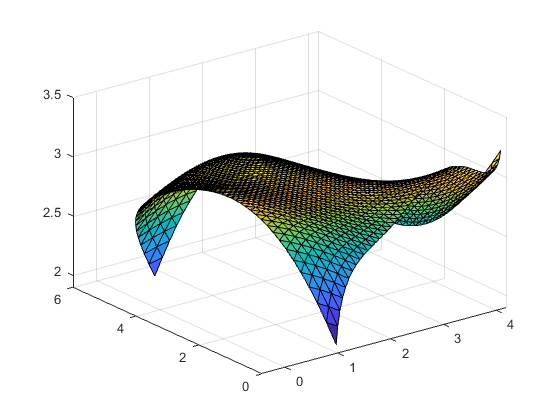
\includegraphics[width=0.45\textwidth]{trikotne_1_6.png}
   }
   \subfigure[Primer stalne trikotne krpe dobljene s parametrom $\alpha = -1/9$]{
   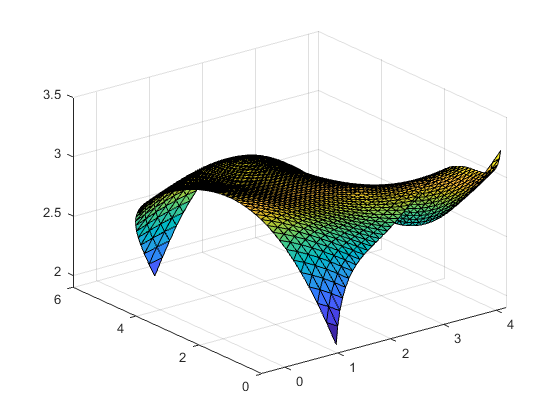
\includegraphics[width=0.45\textwidth]{trikotne_1_9.png}
   }
   
   \subfigure[Primer stalne trikotne krpe dobljene s parametrom $\alpha = 0$]{
   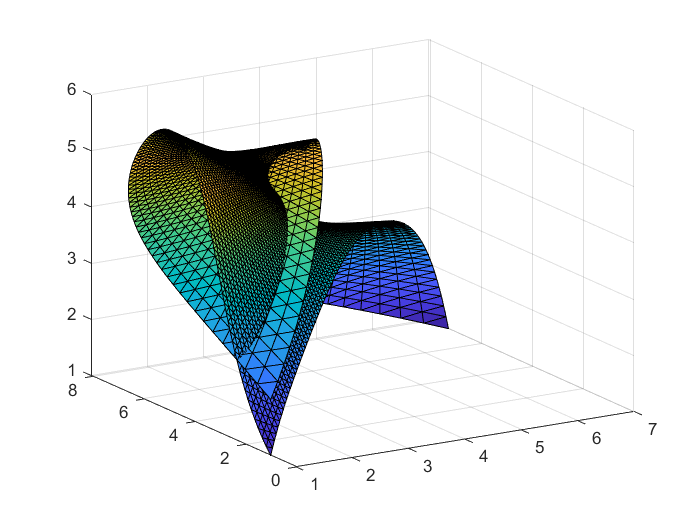
\includegraphics[width=0.5\textwidth]{trikotne_0.png}
   }   
   \caption{Stalne trikotne krpe pridobljene z reševanjem sistemov enačb.}
\label{fig:trikotne}
\end{figure}

Ponovno dobimo pri paramatru $\alpha = 0$ ploskev, 
katere površina je minimizeranan za dano ogrodje krivulj, kar se ponovno vidi iz 
Laplasove parcialne diferencialne enačbe.

\section{Zaključek}

Preoblikovali smo diskretne Consove ploskve in jih posplošili na stalne
ploskve, tako za pravokotne primere kot za trikotne primere. Poslošitev nam omogoča
izdelavo oblik, ki so bolj zaželjene od standardnih Consovih oblik. Ogledali smo 
si vpliv parametrov stalnih Consovih ploskev in jih grafično prikazali.












\newpage


\newpage

\begin{thebibliography}{99}
   \bibitem{DCP}
   G.~Farin, F.~Hansford, \emph{Discrete Coons patches}, 
   % popravi Morgan \& Claypool Publishers, 2018.
\end{thebibliography}
\end{document}